\section{System Overview}
\label{overview}
\noindent
Heimdall has two components: the first is an app installed on a user's mobile device and the second is a Web service that receives install, uninstall and update notifications when these events occur on the device. Upon notification, the server processes all heuristics that apply to the app and generates a set of actions for a system administrator. At this point the system generates a list of recommended actions and sends it over to the Heimdall Mobile App. Our present prototype, includes sample content provider heuristics. The server also allows a system administrator to add more heuristics and add action notifications to be sent to a mobile device in a BYOD scenario.

\begin{figure}[tb]
	\centering
	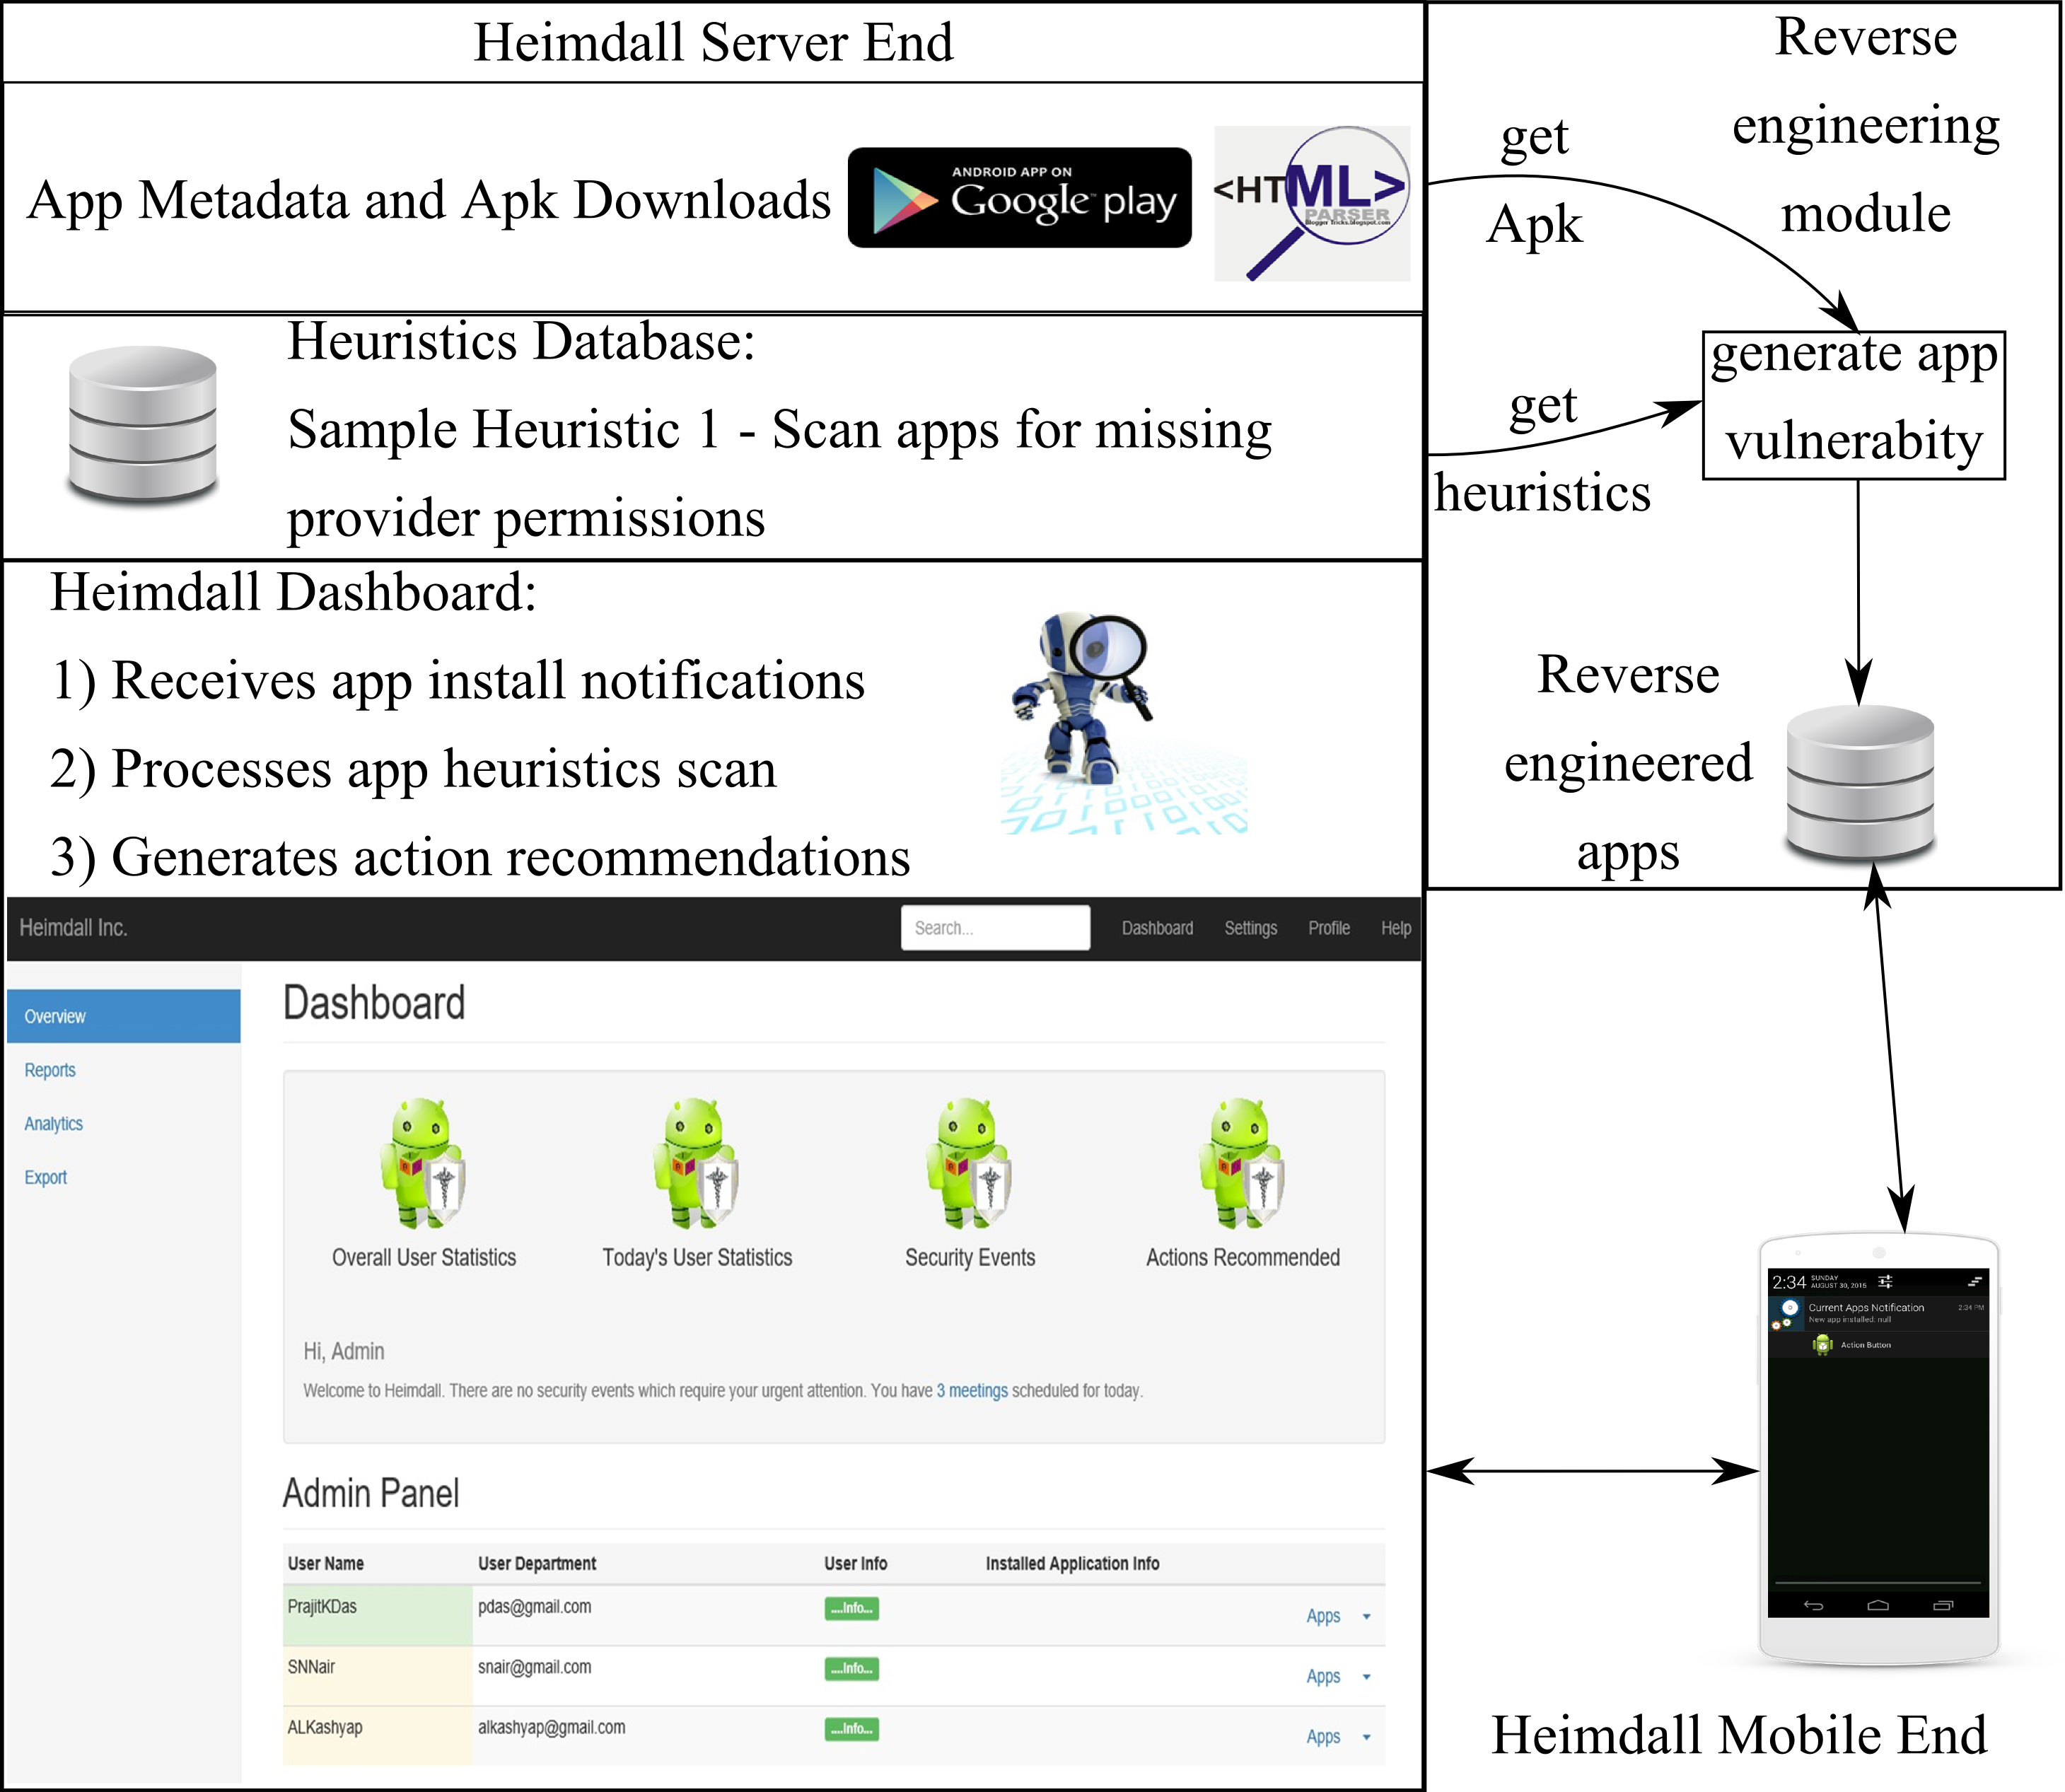
\includegraphics[width=\columnwidth]{images/architecture}
	\caption{System Overview}
	\label{fig:arch}
\end{figure}

\noindent
Heimdall server has two capabilities. It can generate reverse engineered apps that we can test on mobile devices. The reverse engineering process takes into account the heuristics that allow us to detect vulnerability in apps. It can then introduce these vulnerabilities into the repackaged apps. For example we discuss a vulnerability in the next section where content providers on Android could have a potential breach of data. We introduce this vulnerability into any provider associated with apps that we are reverse engineering. We then remove any associated permission and ensure that the ``exported'' tag for the provider is set to true. The primary task of Heimdall is to detect the vulnerabilities in the apps, like the one we just described.

For demonstrating these capabilities, we downloaded about 1500 apps from the Google Play Store and used a tool called apktool~\footnote{A tool for reverse engineering 3rd party, closed, binary Android apps~\url{https://ibotpeaches.github.io/Apktool/}} to decompile the Android binary application packages (apks). We then parse the manifest files to find providers and thus determine whether the apps are vulnerable or not. At the same time if they are not already vulnerable we can introduce the vulnerability and repackage the app for testing purposes. We are working on including more heuristics into Heimdall to make it capable of detecting many more vulnerabilities.